\documentclass{article}
\usepackage{tikz}
\usetikzlibrary{positioning}

\begin{document}

\begin{figure}[h]
    \centering
    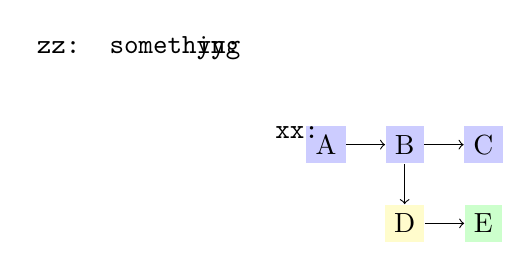
\begin{tikzpicture}[node distance=1cm, auto]
        % Define nodes
        \node (A) [fill=blue!20] {A};
        \node (B) [right of=A, fill=blue!20] {B};
        \node (C) [right of=B, fill=blue!20] {C};
        \node (D) [below of=B, fill=yellow!20] {D};
        \node (E) [right of=D, fill=green!20] {E};

        % Draw edges
        \path[->] (A) edge node {} (B);
        \path[->] (B) edge node {} (C);
        \path[->] (B) edge node {} (D);
        \path[->] (D) edge node {} (E);

        % Caption
        \node [above left=of A] {\texttt{zz: something}};
        \node [above left=of A] {\texttt{yy:}};
        \node [above left=of D] {\texttt{xx:}};
    \end{tikzpicture}
    \caption{Sample Diagram}
    \label{fig:sample_diagram}
\end{figure}

\end{document}